\documentclass[a4paper,11pt]{article}

% Packages essentiels
\usepackage[utf8]{inputenc}
\usepackage[T1]{fontenc}
\usepackage[french]{babel}
\usepackage{lmodern}
\usepackage{microtype}
\usepackage{graphicx}
\usepackage{hyperref}
\usepackage{xcolor}
\usepackage{tcolorbox}
\usepackage{enumitem}
\usepackage{geometry}
\usepackage{fancyhdr}
\usepackage[table]{xcolor}
\usepackage{booktabs}
\usepackage{array}
\usepackage{tabularx}
\usepackage{listings}
\usepackage{fancyvrb}
\usepackage{multicol}

\geometry{margin=2cm, top=2.5cm, bottom=2.5cm}
\setlength{\headheight}{14pt}

\definecolor{titlecolor}{RGB}{0, 90, 160}
\definecolor{sectitlecolor}{RGB}{5, 100, 175}
\definecolor{subsectitlecolor}{RGB}{10, 110, 190}
\definecolor{definitionbg}{RGB}{240, 248, 255}
\definecolor{examplebg}{RGB}{245, 255, 245}
\definecolor{warningbg}{RGB}{255, 245, 245}
\definecolor{benefitbg}{RGB}{255, 253, 235}
\definecolor{codecolor}{RGB}{240, 240, 240}
\definecolor{codekeyword}{RGB}{0, 0, 128}
\definecolor{codestring}{RGB}{163, 21, 21}
\definecolor{codecomment}{RGB}{0, 128, 0}
\definecolor{todobg}{RGB}{255, 235, 235}
\definecolor{collabg}{RGB}{245, 240, 255}

\lstset{
  basicstyle=\ttfamily\footnotesize,
  backgroundcolor=\color{codecolor},
  keywordstyle=\color{codekeyword}\bfseries,
  stringstyle=\color{codestring},
  commentstyle=\color{codecomment}\itshape,
  breaklines=true,
  showstringspaces=false,
  frame=single,
  tabsize=2,
  captionpos=b
}

\pagestyle{fancy}
\fancyhf{}
\fancyhead[L]{\textit{Lab 2 --- L'hexagone}}
\fancyhead[R]{\textit{Architectures Logicielles}}
\fancyfoot[C]{\thepage}
\fancyfoot[L]{\textit{Dr. El Hadji Bassirou TOURE}}
\fancyfoot[R]{\textit{DMI/FST/UCAD}}
\renewcommand{\headrulewidth}{0.4pt}
\renewcommand{\footrulewidth}{0.4pt}

\newtcolorbox{concept}{
  colback=definitionbg, colframe=sectitlecolor,
  title=Concept fondamental, fonttitle=\bfseries
}
\newtcolorbox{intuition}{
  colback=examplebg, colframe=green!75!black,
  title=Intuition, fonttitle=\bfseries
}
\newtcolorbox{exemple}{
  colback=orange!5!white, colframe=orange!75!black,
  title=Exemple, fonttitle=\bfseries, fontupper=\footnotesize
}
\newtcolorbox{pointcle}{
  colback=benefitbg, colframe=orange!70!black,
  title=Point cle a retenir, fonttitle=\bfseries
}
\newtcolorbox{warningbox}{
  colback=warningbg, colframe=red!70!black,
  title=Point d'attention, fonttitle=\bfseries
}
\newtcolorbox{benefitbox}{
  colback=benefitbg, colframe=green!70!black,
  title=Benefice, fonttitle=\bfseries
}
\newtcolorbox{todobox}{
  colback=todobg, colframe=red!60!black,
  title=Tache a realiser, fonttitle=\bfseries\scriptsize, fontupper=\small
}
\newtcolorbox{collabox}{
  colback=collabg, colframe=violet!70!black,
  title=Qui pilote cette section ?, fonttitle=\bfseries\scriptsize, fontupper=\small
}
\newtcolorbox{tagbox}{
  colback=yellow!15, colframe=yellow!50!black,
  title=Jalon Git, fonttitle=\bfseries\scriptsize, fontupper=\small
}

\lstset{
  basicstyle=\tiny\ttfamily,
  keywordstyle=\tiny\ttfamily\bfseries\color{codekeyword},
  commentstyle=\tiny\ttfamily\itshape\color{codecomment},
  stringstyle=\tiny\ttfamily\color{codestring}
}

\usepackage[explicit]{titlesec}
\titleformat{\section}
  {\Large\bfseries\color{titlecolor}}{\thesection}{0.5em}{#1}
\titleformat{\subsection}
  {\large\bfseries\color{sectitlecolor}}{\thesubsection}{0.5em}{#1}
\titleformat{\subsubsection}
  {\normalsize\bfseries\color{subsectitlecolor}}{\thesubsubsection}{0.5em}{#1}

\title{\textcolor{titlecolor}{\Huge\textbf{Lab 2 --- L'hexagone}}\\[0.5em]
       \textcolor{sectitlecolor}{\LARGE Le domaine au centre, la technique en périphérie}}
\author{Dr. El Hadji Bassirou TOURE\\
        Département de Mathématiques et Informatique\\
        Faculté des Sciences et Techniques\\
        Université Cheikh Anta Diop}
\date{Année universitaire 2026--2027}

\begin{document}

\maketitle
\thispagestyle{empty}

\begin{abstract}
\noindent Le Lab 1 a rangé SénResto en couches propres. Ce lab s'attaque au
problème qui reste : le métier dépend toujours de la technique, trois étages
plus bas, et demeure impossible à tester sans base de données. Vous allez
\textbf{inverser cette dépendance} : le domaine définira ses besoins sous
forme de \textbf{ports} (interfaces qui lui appartiennent), et la technique
--- JDBC, REST, notifications --- deviendra un jeu d'\textbf{adaptateurs}
interchangeables. La preuve finale tiendra en une démonstration : remplacer
la base de données par une simple \texttt{Map} en mémoire \textbf{sans
toucher une ligne du domaine}, et voir les tests du métier rendre leur
verdict en deux secondes. Comme toujours : comportement de l'API inchangé,
les 4 tests d'intégration restent verts du début à la fin.
\end{abstract}

\begin{benefitbox}
À l'issue de ce lab, vous saurez :
\begin{itemize}[nosep]
  \item appliquer le principe d'inversion de dépendances --- et expliquer
        pourquoi tout se joue sur la \emph{propriété de l'interface} ;
  \item structurer une application en \textbf{ports \& adaptateurs}
        (architecture hexagonale) ;
  \item écrire des \textbf{tests unitaires du domaine} --- sans Spring,
        sans BDD, sans HTTP ;
  \item démontrer le \textbf{swap d'adaptateur} : changer la technique sans
        toucher au métier.
\end{itemize}
\end{benefitbox}

\begin{warningbox}
\textbf{Prérequis avant la séance :}
\begin{itemize}[nosep]
  \item votre dépôt au tag \texttt{lab2-depart} (= votre \texttt{lab1-final},
        publié à l'ouverture de la séance) ;
  \item \texttt{./mvnw test} vert : \texttt{Tests run: 4, Failures: 0} ;
  \item l'application complète fonctionne (backend + frontend).
\end{itemize}
Si votre groupe n'a pas terminé le Lab 1 : \texttt{git checkout lab2-depart}
sur le dépôt de référence --- personne ne reste au bord de la route.
\end{warningbox}

\tableofcontents
\newpage

% =====================================================================
\section{Le constat : essayez, vous n'y arriverez pas}
% =====================================================================

\begin{intuition}
Avant d'apprendre le remède, ressentez le mal. La direction de SénResto
exige des tests du métier à chaque commit --- rapides, donc unitaires.
Prenez quinze minutes, en groupe, pour \emph{essayer} d'écrire ce test.
L'échec est au programme : c'est lui qui justifie tout le lab.
\end{intuition}

\subsection{L'exercice impossible (15 minutes, en groupe)}

Créez, dans \texttt{src/test/java}, la classe
\texttt{sn.ucad.senresto.service.CommandeServiceTest} et tentez d'écrire
un test de la règle des frais de livraison :

\begin{lstlisting}[language=java]
@Test
void lesFraisSuiventLeQuartier() {
    CommandeService service = new CommandeService(/* ...de quoi ? */);
    // Pour construire CommandeService, il faut : CommandeRepository,
    // RestaurantRepository, LivreurRepository, NotificationService.
    // Pour construire chaque repository, il faut : un JdbcTemplate.
    // Pour un JdbcTemplate, il faut : une DataSource... une BDD qui tourne.
}
\end{lstlisting}

Constatez et notez (vous en aurez besoin pour l'ADR) : pour tester une
\emph{multiplication et une addition}, il faut démarrer toute la pile
technique. Supprimez ensuite ce fichier d'essai --- nous le récrirons
proprement en fin de lab, et il tiendra en dix lignes.

\begin{pointcle}
Le Lab 1 a réglé le \emph{désordre} ; il n'a pas réglé le \textbf{sens des
flèches}. \texttt{CommandeService} $\to$ \texttt{Repository} $\to$
\texttt{JdbcTemplate} $\to$ BDD : tant que le métier pointe vers la
technique, la technique dicte ses conditions au métier.
\end{pointcle}

% =====================================================================
\section{Les concepts : inverser, c'est changer de propriétaire}
% =====================================================================

\begin{concept}
\textbf{Principe d'inversion de dépendances (DIP).} Le code de haut niveau
(le métier) ne dépend pas du code de bas niveau (la technique) : tous deux
dépendent d'\textbf{abstractions}. La subtilité décisive : ces interfaces
appartiennent \textbf{au domaine}, sont écrites dans \emph{son} paquetage
et dans \emph{son} vocabulaire. L'adaptateur technique les
\emph{implémente} --- c'est donc lui qui importe le domaine, et la flèche
de dépendance remonte.
\end{concept}

\begin{figure}[h]
\centering
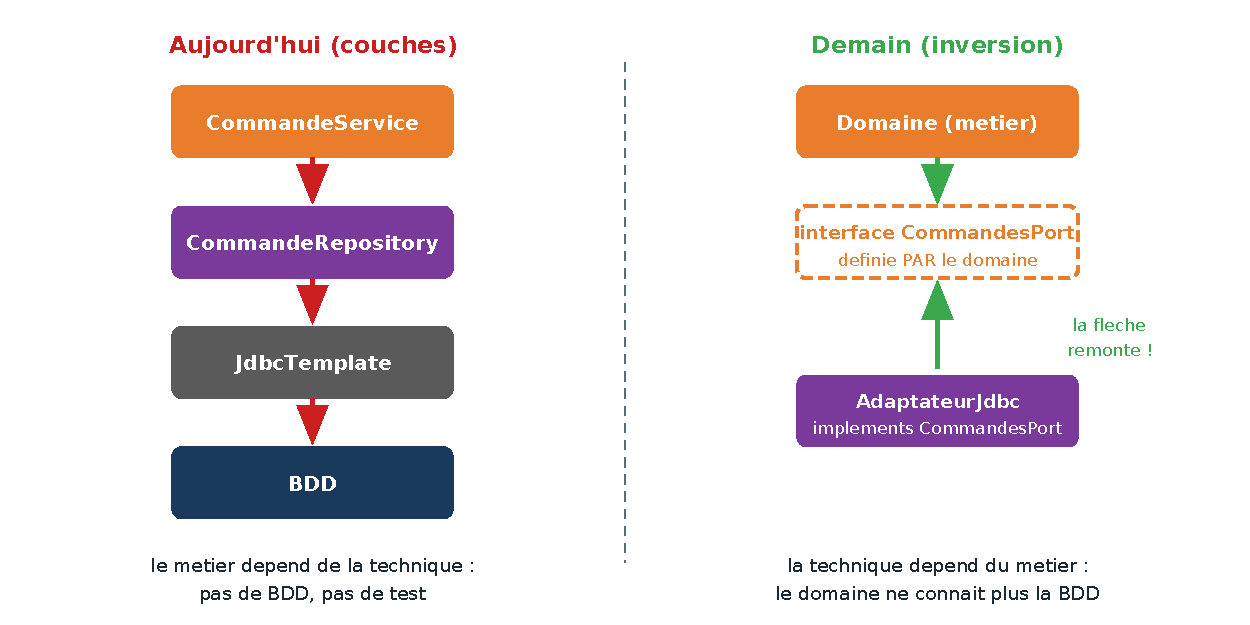
\includegraphics[width=0.62\textwidth]{figs/figC_inversion.pdf}
\caption{L'inversion : la flèche entre métier et persistance change de sens.}
\end{figure}

\begin{concept}
\textbf{Architecture hexagonale (ports \& adaptateurs).} Le domaine vit au
centre, sans aucune dépendance vers l'extérieur --- zéro Spring, zéro SQL,
zéro HTTP. Sa frontière est faite de \textbf{ports} : les interfaces qu'il
définit. Autour, les \textbf{adaptateurs} : entrants (REST traduit HTTP en
appels du domaine) et sortants (JDBC, notifications implémentent les ports).
Règle unique : \textbf{toutes les dépendances pointent vers le centre}.
\end{concept}

\begin{figure}[h]
\centering
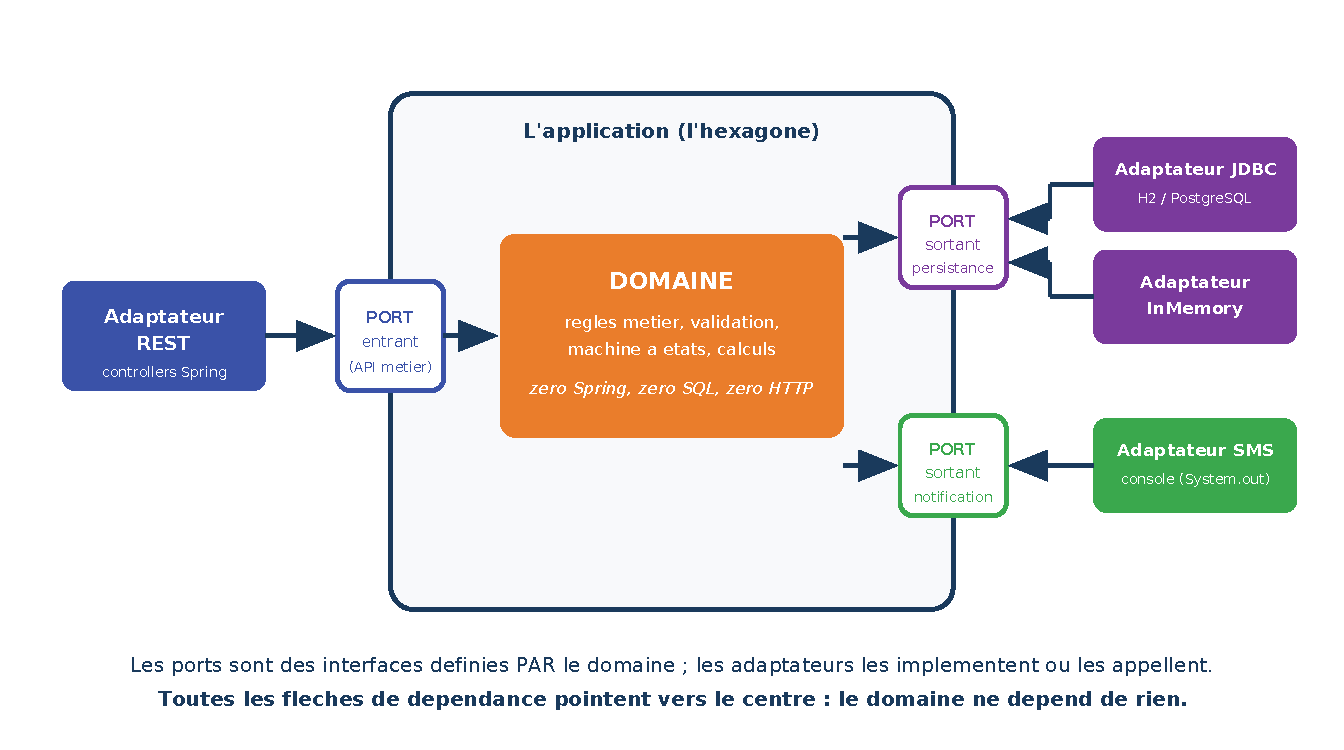
\includegraphics[width=0.80\textwidth]{figs/figD_hexagone.pdf}
\caption{La cible du lab : SénResto en ports \& adaptateurs.}
\end{figure}

\begin{exemple}
Le test du vocabulaire, à appliquer à chaque port que vous écrirez :
lisez-le à voix haute. \texttt{LivreursPort.premierDisponible()} --- du
métier, parfait. \texttt{executerRequeteSql(String sql)} --- de la
technique déguisée en port : refusé. Un port qui mentionne SQL, JSON ou
HTTP est un aveu que la frontière fuit.
\end{exemple}

\subsection{La cible : la nouvelle carte des paquetages}

\begin{lstlisting}[language=bash]
sn/ucad/senresto/
|-- SenRestoApplication.java
|-- domaine/                        <- LE CENTRE : zero import Spring
|   |-- CommandeMetier.java              (ex-CommandeService, sans annotations)
|   |-- RestaurantMetier.java
|   |-- LivreurMetier.java
|   |-- QuartiersDakar.java
|   |-- CalculateurEta.java
|   |-- ValidationException.java  IntrouvableException.java  ConflitException.java
|   \-- port/                       <- les interfaces DU domaine
|       |-- CommandesPort.java
|       |-- RestaurantsPort.java
|       |-- LivreursPort.java
|       \-- NotificationsPort.java
|-- adaptateur/
|   |-- rest/                       <- adaptateur ENTRANT
|   |   |-- SenRestoController.java   GestionnaireErreurs.java
|   |   \-- dto/  (CommandeRequete, ChangementStatutRequete)
|   |-- persistance/                <- adaptateurs SORTANTS (JDBC)
|   |   |-- AdaptateurCommandesJdbc.java      implements CommandesPort
|   |   |-- AdaptateurRestaurantsJdbc.java    implements RestaurantsPort
|   |   \-- AdaptateurLivreursJdbc.java       implements LivreursPort
|   \-- notification/
|       \-- AdaptateurSmsConsole.java         implements NotificationsPort
\-- config/
    \-- ConfigurationDomaine.java   <- Spring instancie le domaine ICI
\end{lstlisting}

\begin{warningbox}
La règle sacrée du lab, vérifiable mécaniquement à tout moment :
\begin{center}
\texttt{grep -r "import org.springframework" backend/src/main/java/sn/ucad/senresto/domaine/}
\end{center}
doit rendre \textbf{zéro ligne}, du premier commit au dernier. Le domaine
ne connaît ni Spring, ni JDBC, ni HTTP --- c'est toute sa valeur.
\end{warningbox}

% =====================================================================
\section{Etape 1 --- Les ports : le domaine dicte ses besoins}
% =====================================================================

\begin{collabox}
\textbf{L'Huissier} pilote : il lit les trois repositories du Lab 1 et en
extrait les signatures \emph{dont le métier a réellement besoin}.
\textbf{Le Notaire} vérifie chaque signature contre son
\texttt{INVENTAIRE-SQL.md} du Lab 1. \textbf{Les autres} préparent leurs
branches d'étape 2. \textbf{Le Doyen} arbitre le vocabulaire des ports.
\end{collabox}

Créez le paquetage \texttt{domaine/port} et les quatre interfaces. Le
patron --- remarquez : \textbf{aucun import}, le vocabulaire du métier,
rien de plus que le besoin :

\begin{lstlisting}[language=java]
package sn.ucad.senresto.domaine.port;

import java.util.List;
import java.util.Map;
import java.util.Optional;

/** Ce dont le metier a besoin pour les livreurs -- rien de plus. */
public interface LivreursPort {
    List<Map<String, Object>> tous();
    Optional<Map<String, Object>> premierDisponible();
    void reserver(long livreurId);
    void liberer(long livreurId);
}
\end{lstlisting}

Sur le même modèle : \texttt{CommandesPort} (inserer, majNumero,
majStatut, majConfirmation, supprimer, toutes, parIdComplet) ;
\texttt{RestaurantsPort} (tous, parId, platsDuRestaurant, platParId) ;
et \texttt{NotificationsPort} (envoyerSms). Les signatures existent déjà dans vos repositories : vous ne
créez pas du code, vous déclarez \emph{à qui il appartient}.

\begin{todobox}
\textbf{À réaliser --- étape 1} (branche \texttt{feature/ports}) :
les quatre interfaces dans \texttt{domaine/port}, relues à voix haute
(test du vocabulaire), compilation verte. C'est une étape courte et
décisive : tout le reste du lab s'appuie dessus.
\end{todobox}

\begin{tagbox}
Compilation verte, vocabulaire validé par le Doyen :
\begin{center}
\texttt{git tag lab2-etape1 \&\& git push origin lab2-etape1}
\end{center}
\end{tagbox}

% =====================================================================
\section{Etape 2 --- Le grand déménagement}
% =====================================================================

\begin{collabox}
\textbf{L'Huissier} déménage le métier dans \texttt{domaine/}.
\textbf{Le Notaire} transforme les repositories en adaptateurs
(\texttt{implements}). \textbf{Le Rédacteur} déplace REST et DTOs dans
\texttt{adaptateur/rest}. \textbf{L'Appariteur} écrit
\texttt{ConfigurationDomaine} et l'adaptateur SMS. \textbf{Le Doyen}
merge dans l'ordre : ports $\to$ domaine $\to$ adaptateurs $\to$ config.
\end{collabox}

\subsection{Le domaine déménage --- et perd ses annotations}

\texttt{CommandeService} devient \texttt{domaine/CommandeMetier} : mêmes
méthodes, mêmes règles, mêmes messages --- mais \textbf{plus aucune
annotation Spring}, et des dépendances déclarées \emph{sur les ports} :

\begin{lstlisting}[language=java]
package sn.ucad.senresto.domaine;

import sn.ucad.senresto.domaine.port.*;
// AUCUN import org.springframework : le domaine est du Java pur.

public class CommandeMetier {

    private final CommandesPort commandes;
    private final RestaurantsPort restaurants;
    private final LivreursPort livreurs;
    private final NotificationsPort notifications;

    public CommandeMetier(CommandesPort commandes, RestaurantsPort restaurants,
                          LivreursPort livreurs, NotificationsPort notifications) {
        this.commandes = commandes;
        this.restaurants = restaurants;
        this.livreurs = livreurs;
        this.notifications = notifications;
    }
    // creer(), confirmer(), changerStatut(), supprimer(), lister(), detail() :
    // le corps des methodes du Lab 1, inchange -- seuls les TYPES des champs
    // ont change : des ports, plus des repositories.
}
\end{lstlisting}

\begin{warningbox}
Question d'équipe (à trancher, puis à consigner dans l'ADR) : où vivent
les DTOs \texttt{CommandeRequete} et \texttt{ChangementStatutRequete} ?
S'ils restent dans l'adaptateur REST, le domaine ne peut pas les recevoir
en paramètre sans dépendre de l'adaptateur --- interdit. Deux options
propres : les déplacer dans le \textbf{domaine} (ce sont des demandes
métier, choix recommandé ici), ou faire traduire l'adaptateur REST vers
des types du domaine. Choisissez en connaissance de cause.
\end{warningbox}

\subsection{Les repositories deviennent des adaptateurs}

Pour le Notaire, l'étape est presque cérémonielle --- le SQL ne change pas
d'une virgule, seule l'\emph{appartenance} change :

\begin{lstlisting}[language=java]
package sn.ucad.senresto.adaptateur.persistance;

import org.springframework.jdbc.core.JdbcTemplate;
import org.springframework.stereotype.Repository;
import sn.ucad.senresto.domaine.port.LivreursPort;
// L'adaptateur importe le domaine : la fleche pointe vers le centre.

@Repository
public class AdaptateurLivreursJdbc implements LivreursPort {
    // ... le contenu exact de LivreurRepository (Lab 1), avec @Override ...
}
\end{lstlisting}

\subsection{Spring assemble l'hexagone --- dans config/, et nulle part ailleurs}

Le domaine n'ayant plus d'annotations, quelqu'un doit l'instancier.
C'est l'unique rôle de la classe \texttt{ConfigurationDomaine},
seul endroit où Spring et le domaine se rencontrent :

\begin{lstlisting}[language=java]
package sn.ucad.senresto.config;

import org.springframework.context.annotation.Bean;
import org.springframework.context.annotation.Configuration;
import sn.ucad.senresto.domaine.*;
import sn.ucad.senresto.domaine.port.*;

@Configuration
public class ConfigurationDomaine {

    @Bean
    public CommandeMetier commandeMetier(CommandesPort commandes,
                                         RestaurantsPort restaurants,
                                         LivreursPort livreurs,
                                         NotificationsPort notifications) {
        return new CommandeMetier(commandes, restaurants, livreurs, notifications);
    }

    @Bean
    public RestaurantMetier restaurantMetier(RestaurantsPort restaurants) {
        return new RestaurantMetier(restaurants);
    }

    @Bean
    public LivreurMetier livreurMetier(LivreursPort livreurs) {
        return new LivreurMetier(livreurs);
    }
}
\end{lstlisting}

Spring injecte automatiquement chaque adaptateur \texttt{@Repository} là où
son \emph{interface} de port est attendue : l'assemblage est déclaratif.
Le controller, lui, change trois types d'import (\texttt{CommandeMetier} au
lieu de \texttt{CommandeService}) et rien d'autre.

\begin{todobox}
\textbf{À réaliser --- étape 2 :}
\begin{itemize}[nosep]
  \item L'Huissier (\texttt{feature/domaine}) : \texttt{CommandeMetier},
        \texttt{RestaurantMetier}, \texttt{LivreurMetier}, exceptions,
        \texttt{QuartiersDakar}, \texttt{CalculateurEta} déménagés dans
        \texttt{domaine/} --- et le \texttt{grep} sacré qui rend zéro ;
  \item Le Notaire (\texttt{feature/adaptateurs-jdbc}) : les trois
        \texttt{AdaptateurXxxJdbc implements XxxPort} ;
  \item Le Rédacteur (\texttt{feature/adaptateur-rest}) : controller,
        gestionnaire d'erreurs et DTOs dans \texttt{adaptateur/rest} (ou
        DTOs dans le domaine selon la décision d'équipe) ;
  \item L'Appariteur (\texttt{feature/config}) :
        \texttt{AdaptateurSmsConsole} et \texttt{ConfigurationDomaine} ;
  \item Le Doyen : merges dans l'ordre, \texttt{./mvnw test} après chacun.
\end{itemize}
\end{todobox}

\begin{tagbox}
\texttt{./mvnw test} vert (4/4), parcours frontend complet, grep sacré à zéro :
\begin{center}
\texttt{git tag lab2-etape2 \&\& git push origin lab2-etape2}
\end{center}
\end{tagbox}

% =====================================================================
\section{Etape finale --- Le swap, et la récompense}
% =====================================================================

\begin{collabox}
\textbf{L'Appariteur} pilote : les adaptateurs in-memory et les nouveaux
tests sont son chef-d'\oe uvre du jour. \textbf{L'Huissier} valide que le
domaine n'a pas bougé d'un caractère. \textbf{Les autres} écrivent chacun
un test unitaire du domaine.
\end{collabox}

\subsection{Les adaptateurs in-memory}

Dans \texttt{src/test/java}, paquetage
\texttt{sn.ucad.senresto.domaine.enmemoire} : quatre classes qui
implémentent les ports avec de simples structures Java. Le patron :

\begin{lstlisting}[language=java]
/** Un "stockage" de commandes : une Map et un compteur. C'est tout. */
public class CommandesEnMemoire implements CommandesPort {

    private final Map<Long, Map<String, Object>> donnees = new LinkedHashMap<>();
    private long prochainId = 1;

    @Override
    public long inserer(String clientNom, String clientTelephone, String clientQuartier,
                        long platId, int quantite, int fraisLivraison, int montantTotal) {
        long id = prochainId++;
        Map<String, Object> c = new LinkedHashMap<>();
        c.put("id", id); c.put("numero", "CMD-TEMP");
        c.put("client_nom", clientNom); c.put("client_telephone", clientTelephone);
        c.put("client_quartier", clientQuartier); c.put("plat_id", platId);
        c.put("quantite", quantite); c.put("frais_livraison", fraisLivraison);
        c.put("montant_total", montantTotal); c.put("statut", "EN_ATTENTE");
        donnees.put(id, c);
        return id;
    }
    // ... les autres methodes : lectures et mises a jour de la Map ...
}
\end{lstlisting}

\subsection{La récompense : le test impossible devient trivial}

Récrivez maintenant le test de la section 1 --- celui qui était
impossible :

\begin{lstlisting}[language=java]
class CommandeMetierTest {

    private CommandeMetier domaine() {
        return new CommandeMetier(new CommandesEnMemoire(),
                new RestaurantsEnMemoire(), new LivreursEnMemoire(),
                new NotificationsEnMemoire());
    }

    @Test
    void lesFraisDeLivraisonSuiventLeQuartier() {
        var commande = domaine().creer(new CommandeRequete(
                "Awa Ba", "771112233", "Ouakam", 1L, 2));
        assertEquals(2500 * 2 + 1500, commande.get("montant_total"));
    }

    @Test
    void confirmerAssigneUnLivreurEtCalculeUnEta() { /* a vous */ }

    @Test
    void uneTransitionInterditeEstRefusee() { /* a vous */ }
}
\end{lstlisting}

Lancez, et savourez le chronomètre : \texttt{./mvnw test} exécute désormais
les 4 tests d'intégration \emph{et} vos tests unitaires --- et ces derniers
rendent leur verdict en \textbf{quelques secondes, sans base de données}.
Faites la démonstration inverse pour la beauté du geste : coupez Docker,
éteignez tout --- les tests du domaine passent toujours.

\begin{figure}[h]
\centering
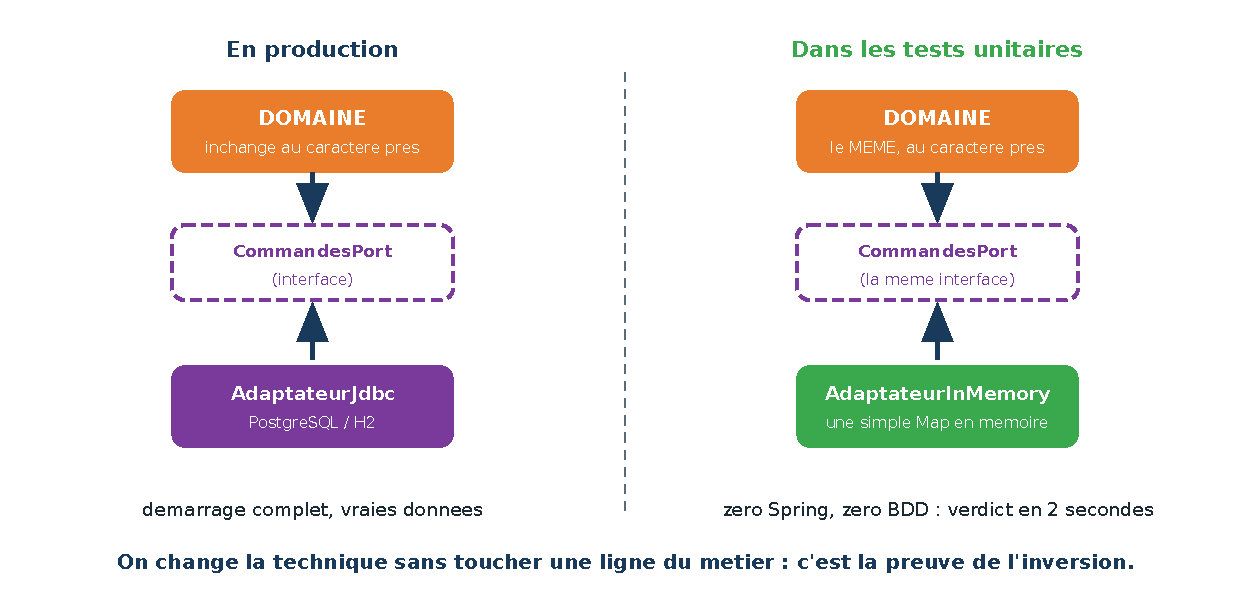
\includegraphics[width=0.72\textwidth]{figs/figE_swap.pdf}
\caption{Le swap : même domaine, technique interchangeable --- la preuve de l'inversion.}
\end{figure}

\begin{pointcle}
Vous venez de constituer la \textbf{pyramide des tests} : nombreux, rapides
et unitaires au centre (le domaine) ; rares, lents et intégrés en périphérie
(le branchement complet). Les deux familles sont complémentaires ---
aucune ne remplace l'autre.
\end{pointcle}

\begin{todobox}
\textbf{À réaliser --- étape finale :}
\begin{itemize}[nosep]
  \item L'Appariteur (\texttt{feature/enmemoire}) : les quatre adaptateurs
        in-memory dans \texttt{src/test/java} ;
  \item Chaque membre : \textbf{au moins un test unitaire} du domaine signé
        de sa main (frais, ETA, transitions, validation, quantités...) ;
  \item L'Huissier : vérification que \texttt{domaine/} est identique entre
        \texttt{lab2-etape2} et \texttt{lab2-final}
        (\texttt{git diff lab2-etape2 -- backend/src/main/java/sn/ucad/senresto/domaine} : vide) ;
  \item Tous : \texttt{./mvnw test} --- intégration 4/4 \emph{et} unitaires
        verts.
\end{itemize}
\end{todobox}

\begin{tagbox}
Le verdict final --- tests d'intégration ET unitaires verts, grep sacré à
zéro, frontend intact :
\begin{center}
\texttt{git tag lab2-final \&\& git push origin lab2-final}
\end{center}
\end{tagbox}

% =====================================================================
\section{Recapitulatif : qui a fait quoi}
% =====================================================================

\begin{center}
\small
\begin{tabular}{p{0.16\textwidth}p{0.24\textwidth}p{0.28\textwidth}p{0.22\textwidth}}
\toprule
\textbf{Rôle} & \textbf{Étape 1} & \textbf{Étape 2} & \textbf{Étape finale} \\
\midrule
Le Doyen & arbitrage du vocabulaire & merges ordonnés, tests & tag final, ADR \\
\addlinespace
L'Huissier & extraction des signatures & déménagement du domaine, grep sacré & domaine gelé (diff vide) \\
\addlinespace
Le Rédacteur & relecture des ports & adaptateur REST, décision DTOs & un test unitaire signé \\
\addlinespace
Le Notaire & vérif. contre l'inventaire SQL & les trois adaptateurs JDBC & un test unitaire signé \\
\addlinespace
L'Appariteur & branches préparées & \texttt{ConfigurationDomaine}, SMS & in-memory + tests unitaires \\
\bottomrule
\end{tabular}
\end{center}

% =====================================================================
\section{L'ADR du jour}
% =====================================================================

L'\textbf{Architecte du jour} rédige et signe l'\textbf{ADR n\up{o}2 :
« Pourquoi inverser les dépendances ? »} (gabarit habituel,
\texttt{docs/adr/adr-002-inversion.md}, avant le tag final). Matière à
alternatives sérieuses : rester en couches et tester le métier avec une
BDD embarquée dédiée aux tests ? Utiliser des mocks (Mockito) sur les
repositories sans inverser quoi que ce soit ? Matière à conséquences
négatives : le coût des interfaces, l'indirection, la
\texttt{ConfigurationDomaine} à maintenir, la discipline du vocabulaire.
Et une exigence de contexte : citer \emph{votre} expérience de la
section 1 --- le test impossible.

% =====================================================================
\section{Livrable et criteres de reussite}
% =====================================================================

\begin{center}
\small
\begin{tabular}{p{0.62\textwidth}p{0.28\textwidth}}
\toprule
\textbf{Critère} & \textbf{Vérification} \\
\midrule
Les 4 tags du lab présents sur le dépôt & \texttt{git tag} \\
Tests d'intégration ET unitaires verts sur \texttt{lab2-final} & \texttt{./mvnw test} \\
Zéro import Spring dans \texttt{domaine/} & le grep sacré \\
Les quatre ports dans \texttt{domaine/port}, vocabulaire métier & relecture \\
Le domaine identique entre etape2 et final & \texttt{git diff} vide \\
Au moins un test unitaire signé par membre & historique Git \\
Frontend intact, parcours complet fonctionnel & démonstration \\
ADR n\up{o}2 signé dans \texttt{docs/adr/} & relecture \\
\bottomrule
\end{tabular}
\end{center}

% =====================================================================
\section{Vers le Lab 3 : la frontière qui manque}
% =====================================================================

Votre hexagone protège le métier de la technique. Mais regardez
\emph{à l'intérieur} du domaine : commandes, restaurants, livreurs,
notifications --- et bientôt le paiement mobile money --- vivent tous dans
le \emph{même} hexagone, libres de s'appeler les uns les autres. Quand
SénResto grandira, qui empêchera le code du Catalogue de fouiller dans
les données du Paiement ? Il manque des frontières \emph{entre les
métiers} --- pas seulement entre le métier et la technique. C'est le
sujet du Lab 3 : le \textbf{monolithe modulaire}, avec Spring Modulith
en gardien automatique des frontières. Votre \texttt{lab2-final} en sera
le point de départ.

\vspace{1em}
\begin{center}
\textit{Fin du Lab 2 --- Dr. El Hadji Bassirou TOURE --- DMI/FST/UCAD}
\end{center}

\end{document}
